\chapter{Recalling items}\label{sec:recall}
In the original TCM model \parencite{Howard2002} the activations $a_i$ of items in the memory is mapped to a recall probability by a softmax function
\begin{equation}
    P(\tcmitem_i | \ctx) = \frac{\exp(2a_i/\tau)}{\sum_j \exp(2a_j/\tau)}
\end{equation}
with a free parameter $\tau$ controlling for the sensitivity.
While this does well in capturing the recall probabilities, it does not provide much insight in how this recall process might be realized neurally.
In an extension of the TCM model \parencite{Sederberg2008} a winner-take-all (WTA) process based on the widely-used leaky, competing accumulator (LCA) model by \textcite{Usher2001} was used.
This works well if the output can be evaluated in a mathematical analysis.
However, within the CUE model other parts of the model need to recognize when a single recall is completed to update the context and reset the recall system.
As I show, this is difficult to do robustly with the LCA model, but more easily accomplished with an alternate WTA mechanism termed the independent accumulator (IA) model.
A comparison of these two networks has also been previously published as \textcite{jangosmann2017}.


\section{Leaky, competing accumulator model}
Given $D$ choices, the leaky, competing accumulator (LCA) model proposed by \textcite{Usher2001} describes the dynamics of $D$ scalar state variables $x_i(t), 1 \leq i \leq D$ as
\begin{equation}
    \od{x_i}{t} = \frac{1}{\tau} \del{u_i(t) -\kappa x_i - \lambda \sum_{j \neq i} x_j}, \quad x_i \geq 0 \label{eqn:lca}
\end{equation}
where $u_i(t)$ are the external inputs, $\kappa$ is the leak rate, $\lambda$ the lateral inhibition, and $\tau$ the integration time-constant.
Each state variable $x_i$ is kept non-negative by setting negative values to zero.
Intuitively, each state variable integrates its input with leak term of $-\kappa x_i$ and provides lateral inhibition to all other state variables.
Given one input $u_i > u_j$ for all $j \neq i$, the state variable $x_i$ will converge to $u_i$ while all other state variables $x_j,\ j \neq i$ will converge to $0$ if $\kappa = \lambda = 1$ (\cref{sec:apdx-wta}).
In the following analysis, $\kappa = \lambda = 1$ will be fixed.
Other choices of $\lambda$ affect the effective integration time-constant $\tau$ and gain on the input, while changing $\beta$ results in undesired behaviour where the history of inputs influences the current choice.

By means of principle 3 of the NEF, the prescribed dynamics can be exactly implemented in the NEF\@.
Here, one ensemble per state variable is used (\cref{fig:lca}) and the gains and biases of the neurons are distributed as described in \cref{sec:thresholding} to ensure the rectification of the state variables.
\begin{figure}
    \begin{captionbeside}{Leaky, competing accumulator (LCA) network\label{fig:lca}.}
        \begin{tikzpicture}[nef, every path/.style={-{Latex}}]
            \matrix [column sep=20, row sep=18] {
                \node (rho1) {$\rho_1$}; & \node (x1) [ens] {$x_1$}; &[20] \node (out1) {}; \\
                \node (rho2) {$\rho_2$}; & \node (x2) [ens] {$x_2$}; & \node (out2) {}; \\
                & \node {$\vdots$}; & \\
                \node (rhoD) {$\rho_D$}; & \node (xD) [ens] {$x_D$}; & \node (outD) {}; \\
            };

            \foreach \i in {1, 2, D} {
                \draw [loop above, min distance=18, in=110, out=70] (x\i) to (x\i);
                \draw (rho\i) to (x\i);
                \draw (x\i) to (out\i);
            }
            \draw (x1) [inhibit, in=20, out=340, distance=15] to (x2);
            \draw (x1) [inhibit, in=20, out=340, distance=30] to (xD);
            \draw (xD) [inhibit, out=35, in=325, distance=30] to (x1);
            \draw (xD) [inhibit, out=35, in=340, distance=15] to (x2);
            \draw (x2) [inhibit, out=40, in=310, distance=8] to (x1);
            \draw (x2) [inhibit, out=320, in=50, distance=8] to (xD);
        \end{tikzpicture}
    \end{captionbeside}
\end{figure}


\section{Independent accumulator model}\label{sec:ia}
The dynamics of the independent accumulator (IA) model are given by
\begin{align}
    \od{x_i}{t} &= \frac{1}{\tau_1} u_i(t) + \frac{1}{\tau_2} \del{\bar{x}_i - \bar{\lambda} \sum_{j \neq i} \bar{x}_j}, \quad x_i \geq 0 \\
    \bar{x}_i &= \Heavi(x_i - \vartheta)
\end{align}
where $u_i(t)$ again gives the external input, $\tau_1$ and $\tau_2$ are feedforward and feedback time-constants, $\bar{\lambda}$ is an inhibition constant, $\Heavi$ is the Heaviside step function, and $\vartheta$ is a threshold.
The Heaviside non-linearity is the crucial difference to the LCA model as we can reduce this equation to \cref{eqn:lca} by setting $\tau = \tau_1$, $k = -\tau_1/\tau_2$, and $\lambda = \bar{\lambda} \tau_1/\tau_2$ when not considering the Heaviside function.
Through the Heaviside function, the accumulators act as perfect (opposed to leaky) and independent integrators.
Only when the threshold $\vartheta$ is reached, the winning choice is stabilized by feedback while all non-winning choices are inhibited.

These dynamics can again be neurally implemented by means of the NEF (\cref{fig:ia}).
While for the LCA model a single layer was sufficient, it is best to use two layers to implement the IA model.
The first layer consists of independent accumulators representing the state variables $x_i$.
This layer projects to the second layer that performs the computation of $\bar{x}_i$ (i.e.\ the Heaviside function).
The second layer projects back to first layer and can be used to read out the output of the network.
\begin{figure}
    \begin{captionbeside}[Independent accumulator (IA) network.]{The independent accumulator (IA) network. The second layer is used to compute the function $\bar{x}_i = \Heavi(x_i - \vartheta)$.\label{fig:ia}}
        \begin{tikzpicture}[nef, every path/.style={-{Latex}}]

            \matrix [column sep=20, row sep=18] {
                \node (rho1) {$\rho_1$}; & \node (x1) [ens] {$x_1$}; &[20] \node 
                (bar-x1) [ens] {$\bar{x}_1$}; & \node (out1) {}; \\
                \node (rho2) {$\rho_2$}; & \node (x2) [ens] {$x_2$}; & \node (bar-x2) 
                [ens] {$\bar{x}_2$}; & \node (out2) {}; \\
                & \node {$\vdots$}; & \node {$\vdots$}; & \\
                \node (rhoD) {$\rho_D$}; & \node (xD) [ens] {$x_D$}; & \node (bar-xD) 
                [ens] {$\bar{x}_D$}; & \node (outD) {}; \\
            };

            \foreach \i in {1, 2, D} {
                \draw [loop above, min distance=18, in=110, out=70] (x\i) to (x\i);
                \draw (rho\i) to (x\i);
                \draw (x\i) [{Latex}-{Latex}] to  (bar-x\i);
                \draw (bar-x\i) to (out\i);
            }
            \foreach \i/\j in {1/2, 1/D, 2/D} {
                \draw (bar-x\i) [inhibit, in=20, out=200]  to (x\j);
            }
            \foreach \i/\j in {2/1, D/1, D/2} {
                \draw (bar-x\i) [inhibit, in=-20, out=160]  to (x\j);
            }

            \node (l1) [above=0.4cm of x1, ext] {Layer 1};
            \node [above=0.4cm of bar-x1, ext] {Layer 2};
            \node [left=0.1cm of l1, ext] {Inputs};
        \end{tikzpicture}
    \end{captionbeside}
\end{figure}

\section{Comparisons of the WTA networks}
The pure analytical description does not tell us which network is better suited for certain tasks.
To compare these networks, I simulate them with an input of $u_i = u - s\del{1 - \krond_{1i}} + \eta_i$, where $u$ is the magnitude of the largest input, $s > 0$ is the target separation, $\krond$ is the Kronecker delta, and $\eta_i$ is Gaussian white noise with a standard deviation of $\sigma$.  (without loss of generality as we can reorder the indices).
The first input is always set to be the target and all other inputs are set to be lower by $s$.
The rationale behind this is that it should present the hardest case because every choice is close to the largest input.
As $s \rightarrow 0$, the problem gets more difficult as the separation to the target shrinks.
Note, that $u$ determines the general baseline of inputs in addition to the value of the largest input.
Furthermore, it is important to consider the influence of noise $\eta_i$ on the robustness of the decision process.

As the input lists to the CUE model are about ten to twelve items, I compare the networks for $D=10$ choices.
To make a fair comparison \num{200}~LIF neurons are used per choice in either model.
In the IA model this means, that the number of neurons is split between the first and second layer.
Here I use \num{150} neurons in the first, and \num{50} neurons in the second layer.
As the first layer is performing the evidence accumulation it needs to more accurate and requires more neural resources.
Due to the lower number of neurons in the output layer, the decoded output has a higher variance.
This, however, is not as relevant as variation of the highest output.
If all other choices do not produce an output, the winning choice can still be clearly identified despite the variance.

Given this basic setup of the comparison, a number of metrics give insight in the performance of the networks.
First, we want the network to reach a \emph{clear decision} which I define as exactly one output being above a threshold of \num{0.15} during the time interval from \SIrange{1}{2}{\second} simulation time, while all other outputs remain below the threshold.
The threshold of \num{0.15} was chosen as it is usually sufficient to tell a zero and non-zero signal apart despite spiking noise (except for very low neuron numbers or firing rates).
This metric requires that the output does not change during the interval as this might cause problems in downstream networks that operate on the output.
Also, with a change in output it would be unclear which output should be taken as the actual decision.
One thing this metric does not take into account is whether the output corresponds to the highest input.
This, whether a decision is \emph{correct}, is the second metric.
But note, that in some situations within a larger scale network a wrong, but clear decision, can be preferable to a decision that tends to be correct, but is unstable.

Two more metrics are used for all trials that reached a clear decision.
The amount of time taken to fulfill the conditions for a clear decision are considered as the \emph{decision time}.
It measures how fast the network is obtaining the decision.
Finally, the networks can produce transient outputs unrelated to the final decision.
A downstream network might consider this output as an actual decision and thus those transient outputs should be as small as possible.
The \emph{highest output of a losing choice} during the whole simulation is taken as a metric for this.


\subsection{Results}
\Cref{fig:ia-clear} shows the proportion of trials that the LCA network reaches a clear decision for different input parameters.
The input magnitude $u$ must be large enough to reliably exceed the \num{0.15} detection threshold under noise.
For $u = 0.2$ and even low amounts of noise the network fails to reach a clear decision.
However, it seems that a too large input magnitude decreases performance as well when we compare the performance for $u=0.6$ and $u=1$.
Increasing the noise standard deviation $\sigma$ or decreasing the target separation $s$, both decrease the performance as this makes the problem harder.
Interestingly, the IA network does not fail to reach a clear decision in any of these conditions.
\begin{figure}
    \centering
    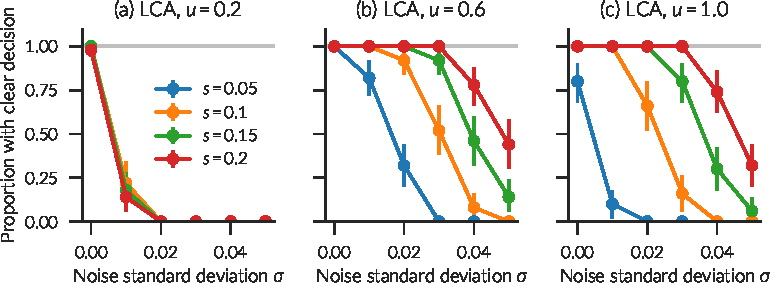
\includegraphics{figures/ia-clear}
    \caption[Proportion of trials with a clear decision for the LCA network.]{Proportion of trials with a clear decision for the LCA network. The data for correct trials is exactly the same. Each plot shows a different input magnitude $u$ and each curve is for a different target separation $s$. The optimum is marked with the gray horizontal line and coincides with the performance of the IA network for clear decisions. Error bars show \SI{95}{\percent} confidence intervals.}\label{fig:ia-clear}
\end{figure}

Moving on to correct decisions, the LCA network always produced the correct output given it produced a clear decision.
The IA network, may produce incorrect outputs despite a clear decision (\cref{fig:ia-correct}).
Again, as the problem gets harder either by decreased target separation or increased noise, the network performance on this metric decreases.
Note that the feedforward integration time-constant can be increased to integrate evidence over a prolonged time period  to increase performance on this metric (right-most panel).
\begin{figure}
    \centering
    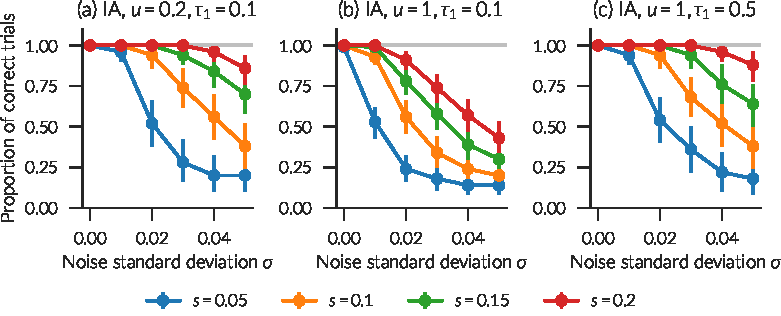
\includegraphics{figures/ia-correct}
    \caption[Proportion of correct trials for the IA network.]{Proportion of correct trials for the IA network. Each plot shows a different combination of input magnitude $u$ and integration time constant $\tau_1$. Each curve shows a different target separation $s$. The optimum is marked with the gray horizontal line. Error bars show \SI{95}{\percent} confidence intervals.}\label{fig:ia-correct}
\end{figure}

This, however, increases the decision times.
These tend to be already slower for the IA network than for the LCA network (\cref{fig:ia-time}).
Additional noise can shorten the decision times in the IA network as it increases the likelihood of an integrator randomly accumulating enough evidence to cross the threshold.
For the LCA network the noise level only has a minor influence on the decision time and was averaged over in the plot.
In other words, noise in the LCA network influences whether a decision can be reached, but not how long it takes to reach a decision if one is reached.
\begin{figure}
    \centering
    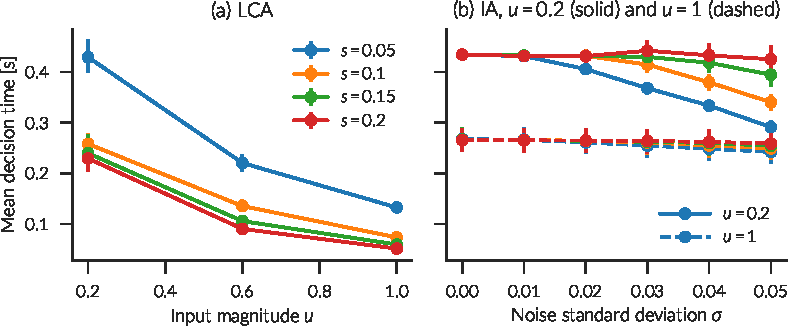
\includegraphics{figures/ia-time}
    \caption[Mean WTA decisions times.]{Mean decision times for the (a) LCA and (b) IA network. Data for the LCA network is shown as depending on the input magnitude $u$ and is averaged over all noise levels $\sigma$ because noise had a minimal effect on decision times. Data fro the IA network is shown as depending on the noise standard deviation $\sigma$ for two input magnitudes of $u = 1$ (dashed lines) and $u = 0.2$ (solid lines). Target separation is indicated by color. Error bars show \SI{95}{\percent} confidence intervals.}\label{fig:ia-time}
\end{figure}

Finally, both networks might produce a transient response that gets worse with increased noise (\cref{fig:ia-transient}).
This is inherent in the LCA network because the state variables are directly used as output.
In the IA network, this transient response is caused when two accumulators cross the threshold in close temporal proximity before the inhibition from the first one can silence the remaining accumulators.
By increasing the feedforward time-constant, this transient response gets reduced as the evidence integration gets slowed down, which temporally stretches out when accumulators cross the threshold.
\begin{figure}
    \centering
    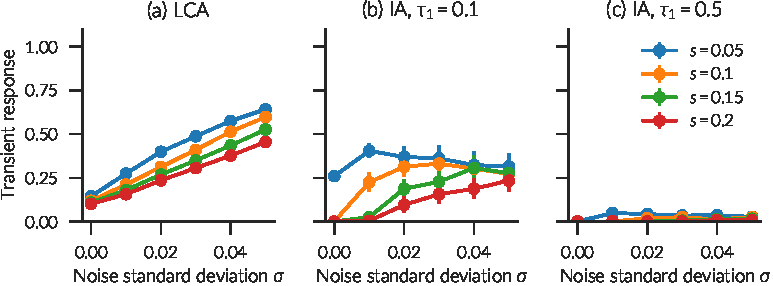
\includegraphics{figures/ia-transient}
    \caption[Transient WTA responses.]{Transient responses (i.e.\ highest output of a non-winning choice) for the WTA networks as depending on the noise standard deviation $\sigma$. Data from the IA network is shown for two integration constants. Each curves shows a different target separation $s$. Error bars show \SI{95}{\percent} confidence intervals.}\label{fig:ia-transient}
\end{figure}


\subsection{Discussion}
Neither network performs better on all metrics.
Thus, each is best suited for a different purpose.
In situations where a continuous adjustment of a decision is necessary, the LCA network is most likely the better choice.
Under noisy conditions it is not necessarily able to produce a stable, clear output, but if a clear output is obtained, it is always correct.
If the input changes, the output adjusts according to the network's time constant and allows for continuous updates.
Unfortunately, this also makes the network susceptible to noise.

The IA network is better for a discrete series of decisions.
It does not produce a continuous output, but waits until the evidence integration threshold is crossed, at which point the network needs to be inhibited to be reset and obtain another decision.
While this produces sequential and discrete decisions, it has the advantage that evidence can be accumulated over a longer time frame to average out noise.
Depending on the choice of the integration time-constant, the IA network either be not as quick or as reliable in identifying the correct winner as the LCA network.
However, it will eventually produces a clear decision that a downstream network can act on (as long as at least one input is strictly positive).
This can be important in a larger scale model where stalling a decision indefinitely can result in a breakdown of model behaviour.
Or in other words, sometimes it is better to act on a wrong decision than to not act all.
For example, in memory recall it might be better to produce a wrong output and continue to recall the next item than indefinitely be trying to recall an item that cannot be recalled.
It is also worth pointing out that the IA network allows for dynamic control of the decision speed by adjusting the $\vartheta$ threshold through a bias input to the second layer.

As mentioned, it is also important to consider the transient outputs of the network within a larger scale model.
Such transient responses are inherent in the LCA model as the state variable is directly used as an output.
One could pass the output through a thresholding layer, but the right choice of threshold is not clear, as the output magnitude depends on the input magnitude.
If the threshold is too low, a transient response would be produced even with the thresholding layer.
If it is too high, small inputs might not produce an output at all.
While the IA can also produce transient responses, these can be reduced to almost zero by a proper selection of the integration time-constant according to the input magnitude and target separation.

By increasing $\tau_1 \rightarrow \infty$, the IA discrimination ability can be increased without bound.
This is sometimes used as argument to criticize these sort of models \parencite[e.g.,][]{Usher2001}, because there is no sensible stopping criterion.
However, this does not consider that there might be a cost to taking more time for a decision.
If that cost is included, then there is a trade-off between accurate decisions and the cost incurred by taking more time to decide.
Furthermore, this argument also assumes perfect integration accuracy, which an actual neural system cannot have due to neural noise and limited neural resources.

To summarize these findings, for the recall of items in memory experiments the IA network is better suited.
Such recall requires discrete decisions and a stable input to downstream motor systems producing the response.
Such a stable input cannot be guaranteed with the LCA network and it proves a challenge to detect when a recall is completed.
\Textcite{Sederberg2008} used the LCA network for modelling the recall, but it is important to highlight that upon reaching the decision threshold, the state variables were immediately set back to zero.
This is easy to do in a pure math model, but when transitioning to a full neural model detecting the decision and resetting the state variables is much more difficult, as it cannot be done instantaneously.

Finally, let us consider biological plausibility briefly.
Both networks where simulated in spiking neurons, which ensures a certain degree of biological plausibility.
Also, accumulation of evidence to a threshold is a well known finding for neurons in LIP \parencite{gold2007,smith2004}.
Often this is assumed to be a gradual integration, but when looking at individual trials instead of the trial-average, a distinct step response becomes evident \parencite{latimer2015}.
This matches the output of the second layer of the IA network.
However, both networks have an integration layer with gradually increasing firing rates, which implies that such neurons should exist too.
Ultimately, it is possible, that the brain employs both networks for different tasks as they have different strengths and weaknesses.


\section{Recall network}\label{sec:recall-net}
The recall network in the CUE model is based on the independent accumulator network.
Each potentially recallable item is regarded as one choice.
An additional \emph{null choice} is added to represent a failed recall.
This is a stand-in for additional items that might be present in the recall network, but have not occurred in the learned list.
It is also a way of providing a time-limit on trying to recall a particular item, and prevents pure noise resulting in a successful recall of one of the learned list items.
The additional choice is fed a constant signal of $\minev$.
Additive Gaussian white noise is applied to each input with zero mean and a standard deviation of $\recnoise$ to account for additional processes that might interfere with the recall process.

Furthermore, the IA network is embedded into further components (\cref{fig:recall}).
First, items are represented as Semantic Pointers, but the IA network needs a separate utility value for each potential choice.
Thus, the incoming connection uses the matrix of the Semantic Pointers of all possible list items as a transform, effectively calculating a dot product between the input signal and each potential item.
These utility values are then rectified to only consider positive evidence.
By subtracting \num{0.1} from the input utilities provided by the OSE output, integration of pure noise from a failed short-term memory recall is prevented.
\begin{figure}
    \centering
    \begin{tikzpicture}[nef]
        \graph [no placement] {
            noise [ext, x=-.5, y=1.5] -> xi/"$x_i$" [ea, x=0, y=0] <-> xib/"$\bar{x}_i$" [ea, x=1.5, y=0];
            oserectshadow/"" [ea, x=-1.5, y=0.5, inner sep=0.25ex];
            tcmrectshadow/"" [ea, x=-1.5, y=-0.5, inner sep=0.25ex];
            OSE [ext, x=-3, y=0.5] -> ["$\mat V$"] oserect/"" [rect, x=-1.5, y=0.5] -> xi;
            b1/"$-0.1$" [ext, x=-2, y=1.5] -> oserect;
            TCM [ext, x=-3, y=-0.5] -> ["$\mat V$"] tcmrect/"" [rect, x=-1.5, y=-0.5] -> xi;

            i1/"" [ens, x=3, y=1];
            xib -> ["$\mat V\Tr$"] g1/"" [ea, x=4, y=0] -> m1/"" [ea, x=5.5, y=0] -> recalled [ext, x=8, y=0];
            m1 -> [bend right, "$-1$"] g1;
            m1 -> [recurrent] m1;

            b2/"$1$" [ext, x=3, y=2] -> i1;

            xib -> ["$x_{\ped{null}}$" {very near end, xshift=3mm}] m2/"" [ens, x=2.5, y=-2.25] -> r2/"" [rect, x=1.5, y=-2.25] -> [inhibit, "$\Heavi(x - 0.3)$" {fill=white, inner sep=0cm, yshift=-2mm}] xi;
            r2 -> [recurrent] r2;

            m1 -> g3/"" [ea, x=5.5, y=-2] -> m3/"" [ea, x=5.5, y=-3.5] -> [bend right] dot [net, x=8, y=-2.5] -> gs3/"" [rect, x=6.5, y=-2.5] -> [inhibit] g3;
            m1 -> [bend left] dot;
            m3 -> [recurrent] m3;
            b3/"$-0.5$" [ext, x=6.5, y=-1.5] -> gs3;

            r4shadow/"" [ea, x=0, y=-4.5, inner sep=0.25ex];
            m3 -> g4/"" [ea, x=3.5, y=-5] -> m4/"" [ea, x=2, y=-5] -> r4/"" [rect, x=0, y=-4.5] -> ["$-6$" xshift=-3mm, bend left] xi;
            m4 -> [recurrent] m4;
            m4 -> ["$-1$", bend left] g4;

            extproc/"ext.\ processing done" [ext, x=3.5, y=-6] -> [inhibit] g4;
        };
        \draw [inhibit] (xib) |- node [above] {\small $\sum$} (i1);
        \draw [-{Latex}] (i1) -| (g1);

        \node (ia) [fit=(xi) (xib), draw, dashed, gray, rounded corners=0.5em, inner sep=0.5em] {};
        \node [above=0cm of ia.north, anchor=south, gray, font={\lato}] {IA};
        
        \node (gm1) [fit={(g1) (m1) (5.5, 0.75)}, draw, dashed, gray, rounded corners=0.5em, inner sep=0.5em] {};
        \node [above=0cm of gm1.north, anchor=south, gray, font={\lato}] {output};

        \node (freset) [fit={(m2) (r2) (2.5, -1.5)}, draw, dashed, gray, rounded corners=0.5em, inner sep=0.5em] {};
        \node [below=0cm of freset.south, anchor=north, gray, font={\lato}] {failed recall reset};

        \node (stage1) [fit=(g3) (m3) (dot) (gs3) (g3) (b3), draw, dashed, gray, rounded corners=0.5em, inner sep=0.5em] {};
        \node [below=0cm of stage1.south, anchor=north, gray, font={\lato}] {recall inhibition stage 1};

        \node (stage2) [fit={(m4) (g4) (2, -4.25)}, draw, dashed, gray, rounded corners=0.5em, inner sep=0.5em] {};
        \node [below=0cm of stage2.north, anchor=south, gray, font={\lato}] {recall inhibition stage 2};
    \end{tikzpicture}    
    \caption[Recall network.]{Recall network. See text for details.}\label{fig:recall}
\end{figure}

The IA network does not produce an output during the evidence accumulation phase.
It is, however, helpful to have a persistent output of the last recalled item (note that this is still different from the output of the LCA network).
This allows for a simpler analysis and can provide potential future downstream networks with a longer lasting input.
To achieve this, the output of the IA network is routed through a gated memory that is only updated when the IA network produces an output.
As the gated memory stores a Semantic Pointer, a transform matrix needs to be applied to the IA output to project the choice back into the Semantic Pointer space.
The updating is controlled by inhibiting the memory gate by default and disinhibiting it (by inhbiting the inhibitory population) when the IA network produces output.

Repetition errors are rarely made in recall experiments.
Thus, it is necessary to inhibit already recalled items.
However, this inhibition should not happen immediately as otherwise the recall output would be inhibited too quickly for the downstream network to act upon.
Thus, a two-stage process is used.
First, an initial working memory population gets immediately updated by feeding in the currently recalled item.
This adds the recalled Semantic Pointer into the representation of items to inhibit.
From that representation and the current recalled item, a dot product is calculated and thresholded at \num{0.5}.
Once the threshold is crossed, the gate to the memory population is inhibited as the new item should be added into the representation, but not completely overwrite it.
The output of that memory population is fed to a gated memory that provides the inhibition to recall in the IA\@.
The gate for this memory is controlled externally and disinhibited once the downstream processing has completed.
Note that the output of that memory population is projected back into utility values and rectified.
This prevents that a negative cosine similarity with one of the vectors stored in the memory population contributes positive evidence.

Finally, the recall network needs to be reset if a recall fails to allow it to continue trying to recall the item for the next position in serial recall.
Here the problem is that if the IA output for a failed recall is directly used to inhibit the IA network to reset it, this also immediately inhibits the output used for the inhibition.
This does not reliably reset the network as the reset signal is disabling itself.
Thus, the signal is fed to an integrator until a threshold is reached and then the signal of the integrator is used to provide an inhibitory pulse to the IA network.
The slower decay of the integrator ensures a sufficient pulse length to restart the recall process.
